\documentclass{beamer}
\usepackage[utf8]{inputenc}
\usepackage{textpos}
\usepackage{csquotes}
\usepackage{booktabs}
\usepackage[twitter]{emoji}

% smile 			\emoji{1F60A}
% tired				\emoji{1F629}
% read heart		\emoji{2764}
% think 			\emoji{1F914}
% fire				\emoji{1F525}
% rolling eyes		\emoji{1F644}
% 100				\emoji{1F4AF}
% joy tears			\emoji{1F602}
% eyes				\emoji{1F440}
% blue heart		\emoji{1F499}
% two hearts		\emoji{1F495}
% crying			\emoji{1F62D}
% black heart		\emoji{1F5A4}
% stars				\emoji{2728}
% sad				\emoji{1F614}
% purple heart		\emoji{1F49C}
% skull				\emoji{1F480}
% christmas tree	\emoji{1F384}
% heart eyes		\emoji{1F60D}
% rolling laugh		\emoji{1F923}

\usetheme{Boadilla}

\renewcommand{\figurename}{Figure}

\makeatletter
\setbeamertemplate{caption}[numbered]
\setbeamertemplate{footline}
{
  \leavevmode%
  \hbox{%
  \begin{beamercolorbox}[wd=.333333\paperwidth,ht=2.25ex,dp=1ex,center]{author in head/foot}%
    \usebeamerfont{author in head/foot}\insertshortauthor%~~\beamer@ifempty{\insertshortinstitute}{}{(\insertshortinstitute)}
  \end{beamercolorbox}%
  \begin{beamercolorbox}[wd=.333333\paperwidth,ht=2.25ex,dp=1ex,center]{title in head/foot}%
    \usebeamerfont{title in head/foot}\insertshorttitle
  \end{beamercolorbox}%
  \begin{beamercolorbox}[wd=.333333\paperwidth,ht=2.25ex,dp=1ex,right]{date in head/foot}%
    \usebeamerfont{date in head/foot}\insertshortdate{}\hspace*{2em}
    \insertframenumber{} / \inserttotalframenumber\hspace*{2ex} 
  \end{beamercolorbox}}%
  \vskip0pt%
}
\makeatother

%\addtobeamertemplate{frametitle}{}{%
%\begin{textblock*}{100mm}(.75\textwidth,-0.6cm)
%	
\includegraphics[height=1cm,width=3.5cm]{img/FER_logo_3.png}
%\end{textblock*}}

\addtobeamertemplate{frametitle}{}{%
	\begin{textblock*}{100mm}(.89\textwidth,-0.7cm)
		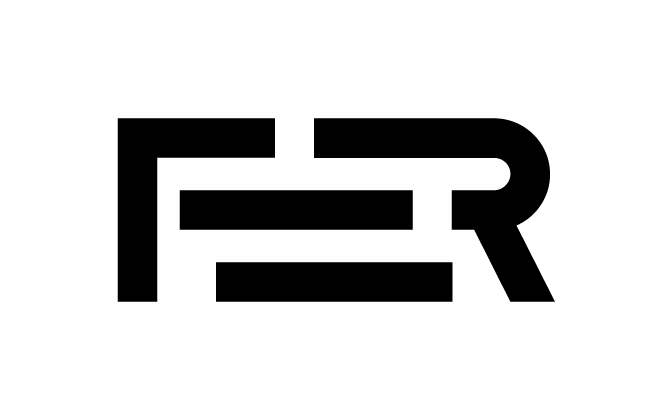
\includegraphics[scale=0.07]{img/FER_logo_1.png}
\end{textblock*}}

\title{Why is emoji prediction difficult?}
\subtitle{TAR project}
\author{Matija Bertović, Antun Magdić, Ante Žužul}
\institute{University of Zagreb \\ Faculty of Electrical Engineering and Computing}
\date{\today}

\begin{document}

\maketitle

\begin{frame}{}
	\begin{displayquote}
		This song is lit! \pause \emoji{1F525} \pause
	\end{displayquote}
	\begin{displayquote}
		And to all, a Merry Christmas! \pause \emoji{1F384} \pause
	\end{displayquote}
	\begin{displayquote}
		I need new friends... \pause \emoji{1F614} \pause \emoji{1F602} \pause
	\end{displayquote}
	\begin{displayquote}
		I'm so happy to have you \pause \emoji{2764} \emoji{1F495} \emoji{1F499} \emoji{1F49C} \emoji{1F60D}
	\end{displayquote}
\end{frame}



\begin{frame}{Dataset}
	\begin{itemize}
		\item 10 million tweets collected
		\item Only tweets with single emoji kept
		\item Final data: $200\,000$ tweets ($20 \times 10\,000$)
		\item Train: $120\,000$, validation: $40\,000$, test: $40\,000$ (all balanced) 
		\item Tweet text $\mapsto$ emoji
	\end{itemize}
\end{frame}


\begin{frame}{Experiment 1}
	\begin{columns}
		\column{0.55\textwidth}
		\begin{itemize}
			\item We compare various models:
			\begin{itemize}
				\item Na\"ive Bayes (NB)
				\item Logistic regression (LR)
				\item Feed forward neural network (NN)
				\item Bidirectional LSTM (BLSTM)
			\end{itemize}
			\item GloVe vs TF-IDF
			\item Word order
			\item Na\"ive assumption
		\end{itemize}
		\column{0.45\textwidth}
		\begin{table}
			\begin{center}
				\begin{tabular}{lr}
					\toprule
					Model & Accuracy (\%) \\
					\midrule
					NB        & 51.15 \\
					LR GloVe  & 33.78 \\
					LR TF-IDF & 53.35 \\
					NN GloVe  & 45.67 \\
					NN TF-IDF & 51.05 \\
					BLSTM     & 51.40 \\
					\bottomrule
				\end{tabular}
			\end{center}
		\end{table}
	\end{columns}	
\end{frame}

\begin{frame}{Experiment 1}
	\begin{figure}
		\begin{center}
			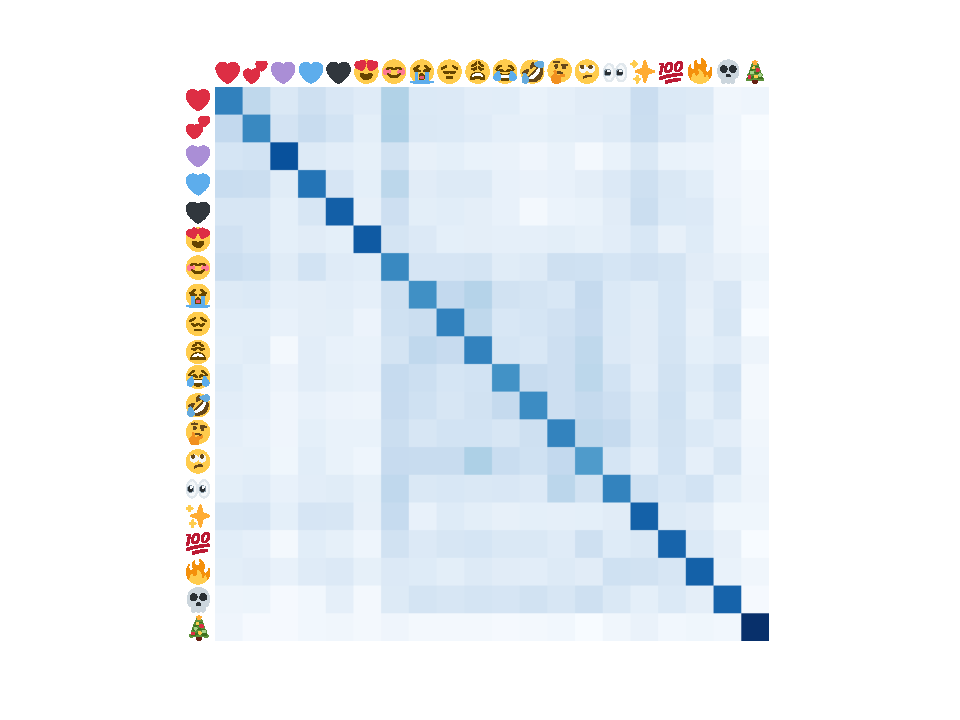
\includegraphics[width=0.6\columnwidth]{img/confusion_matrix.pdf}
		\end{center}
	\end{figure}
\end{frame}

\begin{frame}{Experiment 2}
	\begin{itemize}
		\item K-Means with GloVe (50 clusters)
	\end{itemize}
	\begin{figure}
		\begin{center}
			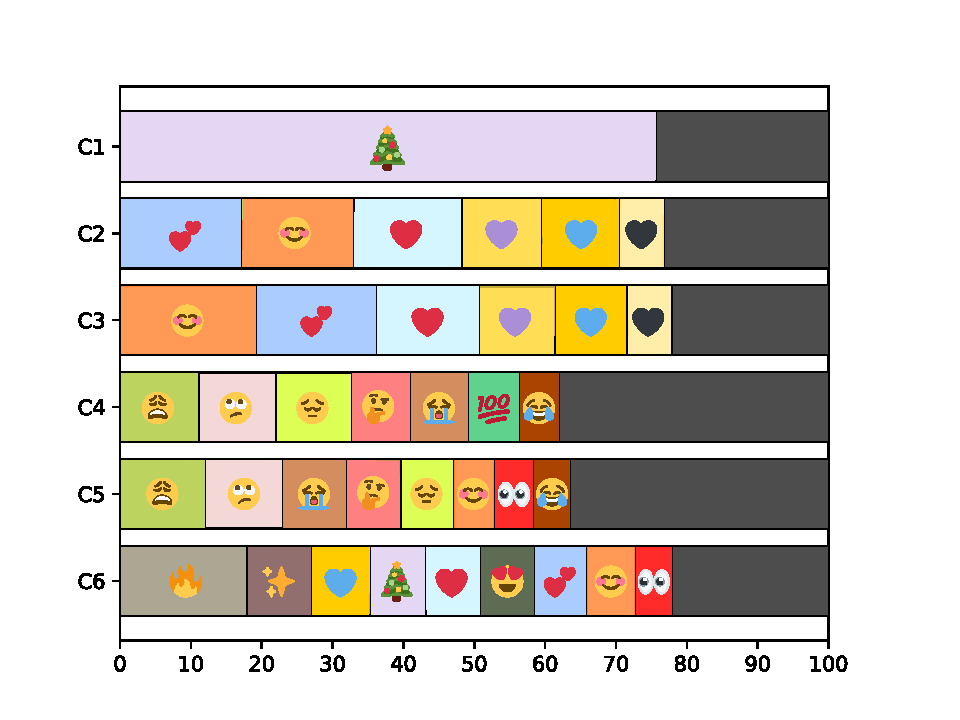
\includegraphics[width=0.6\columnwidth]{img/clusters.pdf}
		\end{center}
	\end{figure}
\end{frame}

\begin{frame}{Conclusion}
	\begin{itemize}
		\item Main difficulties:
		\begin{itemize}
			\item Synonymy among emojis
			\item Subjective meanings
			\item Sarcasm
		\end{itemize}
		\item More information is needed for better performance
	\end{itemize}
\end{frame}

\end{document}